\documentclass[twoside]{book}

% Packages required by doxygen
\usepackage{fixltx2e}
\usepackage{calc}
\usepackage{doxygen}
\usepackage[export]{adjustbox} % also loads graphicx
\usepackage{graphicx}
\usepackage[utf8]{inputenc}
\usepackage{makeidx}
\usepackage{multicol}
\usepackage{multirow}
\PassOptionsToPackage{warn}{textcomp}
\usepackage{textcomp}
\usepackage[nointegrals]{wasysym}
\usepackage[table]{xcolor}

% Font selection
\usepackage[T1]{fontenc}
\usepackage[scaled=.90]{helvet}
\usepackage{courier}
\usepackage{amssymb}
\usepackage{sectsty}
\renewcommand{\familydefault}{\sfdefault}
\allsectionsfont{%
  \fontseries{bc}\selectfont%
  \color{darkgray}%
}
\renewcommand{\DoxyLabelFont}{%
  \fontseries{bc}\selectfont%
  \color{darkgray}%
}
\newcommand{\+}{\discretionary{\mbox{\scriptsize$\hookleftarrow$}}{}{}}

% Page & text layout
\usepackage{geometry}
\geometry{%
  a4paper,%
  top=2.5cm,%
  bottom=2.5cm,%
  left=2.5cm,%
  right=2.5cm%
}
\tolerance=750
\hfuzz=15pt
\hbadness=750
\setlength{\emergencystretch}{15pt}
\setlength{\parindent}{0cm}
\setlength{\parskip}{3ex plus 2ex minus 2ex}
\makeatletter
\renewcommand{\paragraph}{%
  \@startsection{paragraph}{4}{0ex}{-1.0ex}{1.0ex}{%
    \normalfont\normalsize\bfseries\SS@parafont%
  }%
}
\renewcommand{\subparagraph}{%
  \@startsection{subparagraph}{5}{0ex}{-1.0ex}{1.0ex}{%
    \normalfont\normalsize\bfseries\SS@subparafont%
  }%
}
\makeatother

% Headers & footers
\usepackage{fancyhdr}
\pagestyle{fancyplain}
\fancyhead[LE]{\fancyplain{}{\bfseries\thepage}}
\fancyhead[CE]{\fancyplain{}{}}
\fancyhead[RE]{\fancyplain{}{\bfseries\leftmark}}
\fancyhead[LO]{\fancyplain{}{\bfseries\rightmark}}
\fancyhead[CO]{\fancyplain{}{}}
\fancyhead[RO]{\fancyplain{}{\bfseries\thepage}}
\fancyfoot[LE]{\fancyplain{}{}}
\fancyfoot[CE]{\fancyplain{}{}}
\fancyfoot[RE]{\fancyplain{}{\bfseries\scriptsize Generated by Doxygen }}
\fancyfoot[LO]{\fancyplain{}{\bfseries\scriptsize Generated by Doxygen }}
\fancyfoot[CO]{\fancyplain{}{}}
\fancyfoot[RO]{\fancyplain{}{}}
\renewcommand{\footrulewidth}{0.4pt}
\renewcommand{\chaptermark}[1]{%
  \markboth{#1}{}%
}
\renewcommand{\sectionmark}[1]{%
  \markright{\thesection\ #1}%
}

% Indices & bibliography
\usepackage{natbib}
\usepackage[titles]{tocloft}
\setcounter{tocdepth}{3}
\setcounter{secnumdepth}{5}
\makeindex

% Hyperlinks (required, but should be loaded last)
\usepackage{ifpdf}
\ifpdf
  \usepackage[pdftex,pagebackref=true]{hyperref}
\else
  \usepackage[ps2pdf,pagebackref=true]{hyperref}
\fi
\hypersetup{%
  colorlinks=true,%
  linkcolor=blue,%
  citecolor=blue,%
  unicode%
}

% Custom commands
\newcommand{\clearemptydoublepage}{%
  \newpage{\pagestyle{empty}\cleardoublepage}%
}

\usepackage{caption}
\captionsetup{labelsep=space,justification=centering,font={bf},singlelinecheck=off,skip=4pt,position=top}

%===== C O N T E N T S =====

\begin{document}

% Titlepage & ToC
\hypersetup{pageanchor=false,
             bookmarksnumbered=true,
             pdfencoding=unicode
            }
\pagenumbering{roman}
\begin{titlepage}
\vspace*{7cm}
\begin{center}%
{\Large My Project }\\
\vspace*{1cm}
{\large Generated by Doxygen 1.8.11}\\
\end{center}
\end{titlepage}
\clearemptydoublepage
\tableofcontents
\clearemptydoublepage
\pagenumbering{arabic}
\hypersetup{pageanchor=true}

%--- Begin generated contents ---
\chapter{Namespace Index}
\section{Packages}
Here are the packages with brief descriptions (if available)\+:\begin{DoxyCompactList}
\item\contentsline{section}{\hyperlink{namespace_a_l_projet2017_a_l}{A\+L\+Projet2017\+AL} }{\pageref{namespace_a_l_projet2017_a_l}}{}
\end{DoxyCompactList}

\chapter{Hierarchical Index}
\section{Class Hierarchy}
This inheritance list is sorted roughly, but not completely, alphabetically\+:\begin{DoxyCompactList}
\item Http\+Application\begin{DoxyCompactList}
\item \contentsline{section}{A\+L\+Projet2017\+A\+L.\+Mvc\+Application}{\pageref{class_a_l_projet2017_a_l_1_1_mvc_application}}{}
\end{DoxyCompactList}
\item \contentsline{section}{A\+L\+Projet2017\+A\+L.\+Startup}{\pageref{class_a_l_projet2017_a_l_1_1_startup}}{}
\end{DoxyCompactList}

\chapter{Class Index}
\section{Class List}
Here are the classes, structs, unions and interfaces with brief descriptions\+:\begin{DoxyCompactList}
\item\contentsline{section}{\hyperlink{class_a_l_projet2017_a_l_1_1_mvc_application}{A\+L\+Projet2017\+A\+L.\+Mvc\+Application} }{\pageref{class_a_l_projet2017_a_l_1_1_mvc_application}}{}
\item\contentsline{section}{\hyperlink{class_a_l_projet2017_a_l_1_1_startup}{A\+L\+Projet2017\+A\+L.\+Startup} }{\pageref{class_a_l_projet2017_a_l_1_1_startup}}{}
\end{DoxyCompactList}

\chapter{Namespace Documentation}
\hypertarget{namespace_a_l_projet2017_a_l}{}\section{A\+L\+Projet2017\+AL Namespace Reference}
\label{namespace_a_l_projet2017_a_l}\index{A\+L\+Projet2017\+AL@{A\+L\+Projet2017\+AL}}
\subsection*{Classes}
\begin{DoxyCompactItemize}
\item 
class \hyperlink{class_a_l_projet2017_a_l_1_1_mvc_application}{Mvc\+Application}
\item 
class \hyperlink{class_a_l_projet2017_a_l_1_1_startup}{Startup}
\end{DoxyCompactItemize}

\chapter{Class Documentation}
\hypertarget{class_a_l_projet2017_a_l_1_1_mvc_application}{}\section{A\+L\+Projet2017\+A\+L.\+Mvc\+Application Class Reference}
\label{class_a_l_projet2017_a_l_1_1_mvc_application}\index{A\+L\+Projet2017\+A\+L.\+Mvc\+Application@{A\+L\+Projet2017\+A\+L.\+Mvc\+Application}}
Inheritance diagram for A\+L\+Projet2017\+A\+L.\+Mvc\+Application\+:\begin{figure}[H]
\begin{center}
\leavevmode
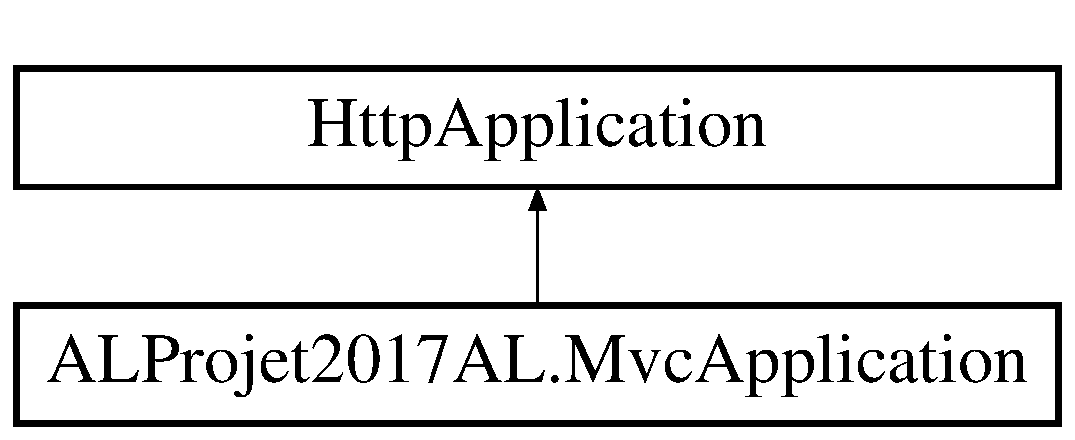
\includegraphics[height=2.000000cm]{class_a_l_projet2017_a_l_1_1_mvc_application}
\end{center}
\end{figure}
\subsection*{Protected Member Functions}
\begin{DoxyCompactItemize}
\item 
void {\bfseries Application\+\_\+\+Start} ()\hypertarget{class_a_l_projet2017_a_l_1_1_mvc_application_aa7f4a7352bf6be8138289267920d3d66}{}\label{class_a_l_projet2017_a_l_1_1_mvc_application_aa7f4a7352bf6be8138289267920d3d66}

\end{DoxyCompactItemize}


The documentation for this class was generated from the following file\+:\begin{DoxyCompactItemize}
\item 
Global.\+asax.\+cs\end{DoxyCompactItemize}

\hypertarget{class_a_l_projet2017_a_l_1_1_startup}{}\section{A\+L\+Projet2017\+A\+L.\+Startup Class Reference}
\label{class_a_l_projet2017_a_l_1_1_startup}\index{A\+L\+Projet2017\+A\+L.\+Startup@{A\+L\+Projet2017\+A\+L.\+Startup}}
\subsection*{Public Member Functions}
\begin{DoxyCompactItemize}
\item 
void {\bfseries Configuration} (I\+App\+Builder app)\hypertarget{class_a_l_projet2017_a_l_1_1_startup_a15fe90123f2b5a8e5b8e3c2294391500}{}\label{class_a_l_projet2017_a_l_1_1_startup_a15fe90123f2b5a8e5b8e3c2294391500}

\end{DoxyCompactItemize}


The documentation for this class was generated from the following file\+:\begin{DoxyCompactItemize}
\item 
Startup.\+cs\end{DoxyCompactItemize}

%--- End generated contents ---

% Index
\backmatter
\newpage
\phantomsection
\clearemptydoublepage
\addcontentsline{toc}{chapter}{Index}
\printindex

\end{document}
